\documentclass[11pt,psfig]{article}
\usepackage{epsfig}
\usepackage{times}
\usepackage{amssymb}
\usepackage{float}

\newcount\refno\refno=1
\def\ref{\the\refno \global\advance\refno by 1}
\def\ux{\underline{x}}
\def\uw{\underline{w}}
\def\bw{\underline{w}}
\def\ut{\underline{\theta}}
\def\umu{\underline{\mu}} 
\def\bmu{\underline{\mu}} 
\def\be{p_e^*}
\newcount\eqnumber\eqnumber=1
\def\eq{\the \eqnumber \global\advance\eqnumber by 1}
\def\eqs{\eq}
\def\eqn{\eqno(\eq)}

 \pagestyle{empty}
\def\baselinestretch{1.1}
\topmargin1in \headsep0.3in
\topmargin0in \oddsidemargin0in \textwidth6.5in \textheight8.5in
\begin{document}
\setlength{\parskip}{1.2ex plus0.3ex minus 0.3ex}


\thispagestyle{empty} \pagestyle{myheadings} \markright{3D Reconstruction of Collagen Fibers}



\title{3D Reconstruction of Collagen Fibers in Cornea}
\author{Zachary DeStefano}
\date{Due Date: June 13, 2014}

\maketitle

\vfill\eject

\newpage

\section{Introduction}

I work in the graphics group with Gopi and Aditi. The group was approached by the Department of Ophthalmology to see if we can reconstruct various parts of the eye using the images provided. I decided to work on reconstructing collagen fibers in the cornea. This mean taking cross-sectional images of them and using that to reconstruct them in a 3D virtual environment. The important aspects of the fibers include shape and size so I just had to locate them in each picture and compile the results together. This also meant that I just had to worry about the brightness value of each pixel and not its RGB vector. The images are somewhat noisy and grainy and the fibers vary in shape and thickness so I had to use a variation of clustering and filtering in order to accurately locate them. Once located, I put the segmentation results into a volumetric data set and used a volume renderer to display it. Here are the steps at a glance that I will go into detail on: \\
\\
1. Do Initial Smoothing of the Image \\
2. Do Clustering to get the fibers\\
3. Smooth the segmented image\\
4. Compare image to previous one and put results into 3D data set\\
5. Add image from step 3 into data set\\
6. Repeat Steps 1-5 for all images in data set\\
7. Use Volume Renderer to show the images in a 3D environment\\
\\
There was an attempted step here of trying to align the images together. I tried various methods to see what the best overlap would be between segmented images but in the end, it made sense to just overlay the images on top of each other without doing any transformations of them. 

\section{Initial Smoothing Step}

For the initial smoothing, I tested out filters that would make the image look less grainy than the original image. I was aiming for a filter that would make the image look like it was a series of bands of black and white. That way whatever clustering algorithm I was using would have an easier time locating the fibers. I tried a Gaussian filter and a median filter but those did not work as well as the simple averaging filter. This is likely because averaging the pixels is more likely to create uniform bands across the image.\\
\\
In order to show the comparison of different filters, here is first the original image to be smoothed.
\begin{figure}[H]
\centering
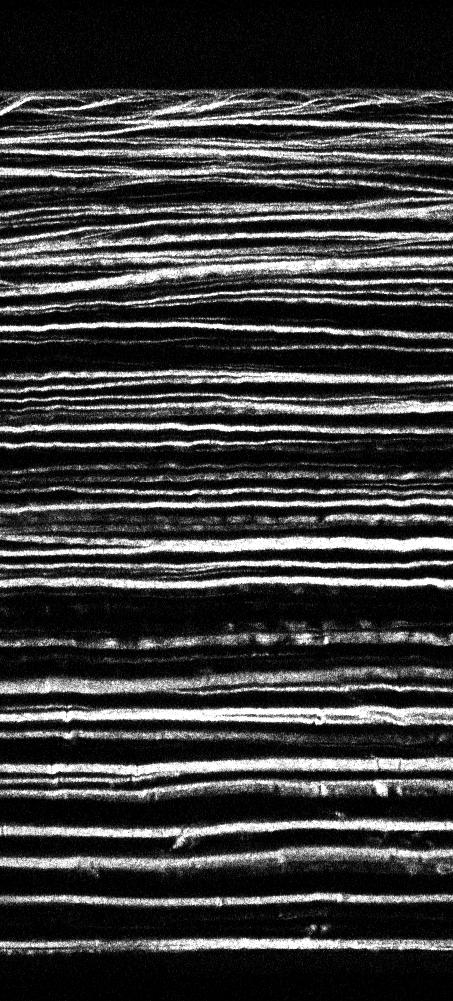
\includegraphics[height=5in]{image1.jpg}
\caption{An example image to be smoothed}
\end{figure}
Here is a pictures of the results of the three different filters.
\begin{figure}[H]
\centering
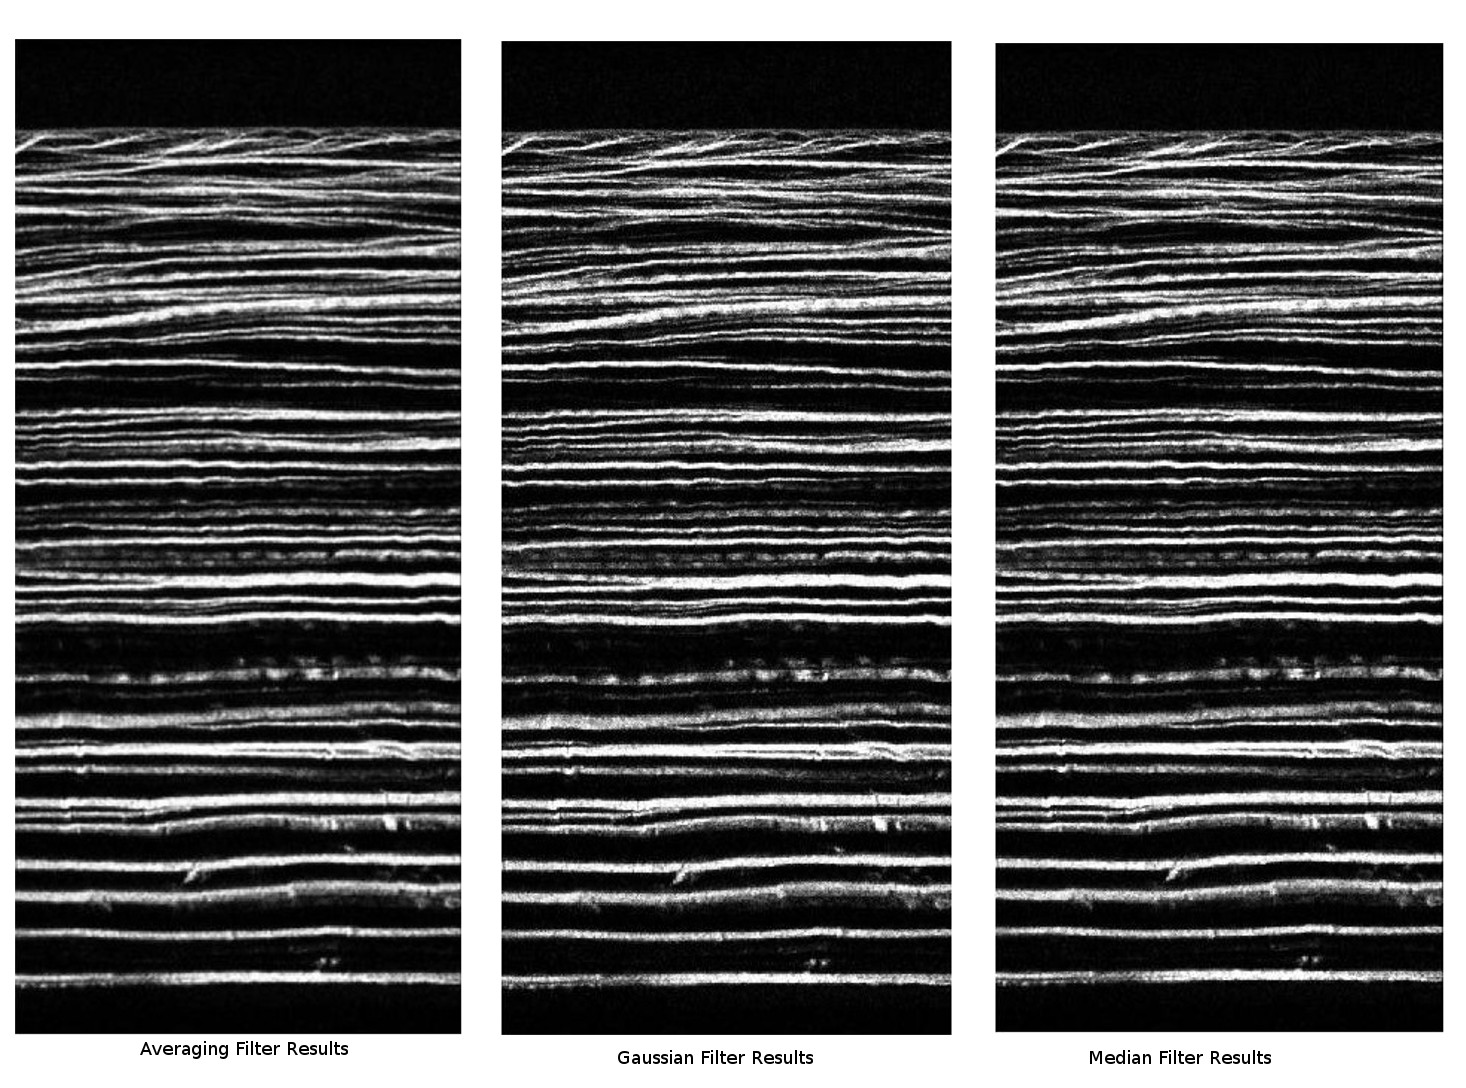
\includegraphics[height=5in]{initialSmoothComparisonPic.jpg}
\caption{The three different initial smoothings done}
\end{figure}

\section{Clustering Step}

This was the most difficult and most important part of the project. Locating the fibers is all about clustering together the different regions of the image where the brightness is high. This was especially difficult for this problem due to the variation in the fibers. The thin fibers at the top were especially easy to miss. With this in mind, I tried the EM algorithm, the min-cut algorithm for MRF, k-Means, simple thresholding, as well as object correlation, and in the end k-Means performed the best. 

\subsection{Simple Thresholding}
I first tried simple thresholding, where any brightness value over a certain amount was classified as a fiber. While this produces some good results, it was not taking spatial proximity into account in the clustering, which is important for this problem. After trying thresholding though, it turned out that $0.3$ was a good classification boundary and I ended up using that when classifying clusters generated by other methods. \\
\begin{figure}[H]
\centering
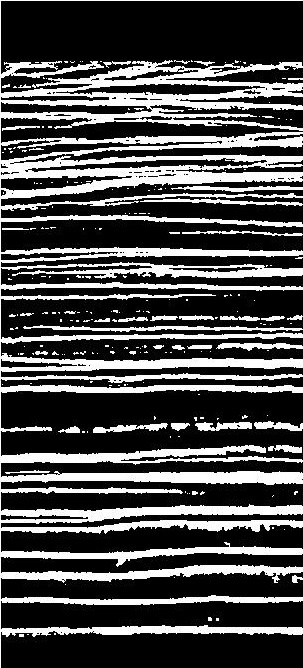
\includegraphics[height=5in]{thresholdSegmentationResult.jpg}
\caption{The segmentation result with simple thresholding}
\end{figure}

\subsection{Simple k-Means}
I tried k-Means with just the brightness values. I used $k=2$ so that it would group it into one cluster that is not a fiber and one that is a fiber. The result was good but there was a lot of noise in the clustering likely due to the fact that it was not taking into account spatial proximity. I decided to try other methods that would be taking spatial proximity into account. Below is the result of the initial k-Means clustering where the greater brightness cluster is colored white and the lower brightness cluster is colored black. 

\begin{figure}[H]
\centering
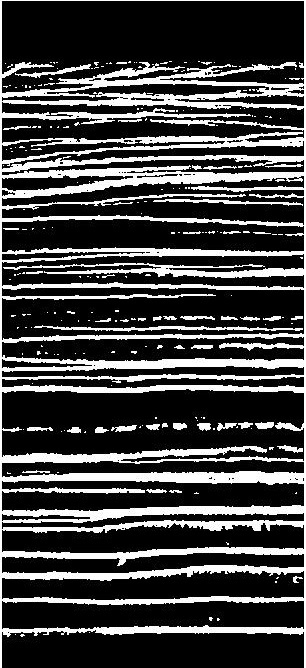
\includegraphics[height=5in]{Initial_kMeansSegmentationResult.jpg}
\caption{k-Means result when k=2}
\end{figure}

\subsection{k-Means on spatial and brightness data}

When I tried k-Means but with $k=30$ and vectors which consisted of a normalized $x$ and $y$ value as well as brightness, I ended up with very nice looking fibers. Around the top of the image, the fibers start to thin out so they are harder to detect, but k-Means was still able to detect them. From my experience with thresholding, I used $0.3$ as the classification boundary between clusters classified as representing regions that were fibers and ones that were not fibers. Below is the result of running k-Means in this manner with the raw clusters displayed on the left and the segmented clusters displayed on the right.

\begin{figure}[H]
\centering
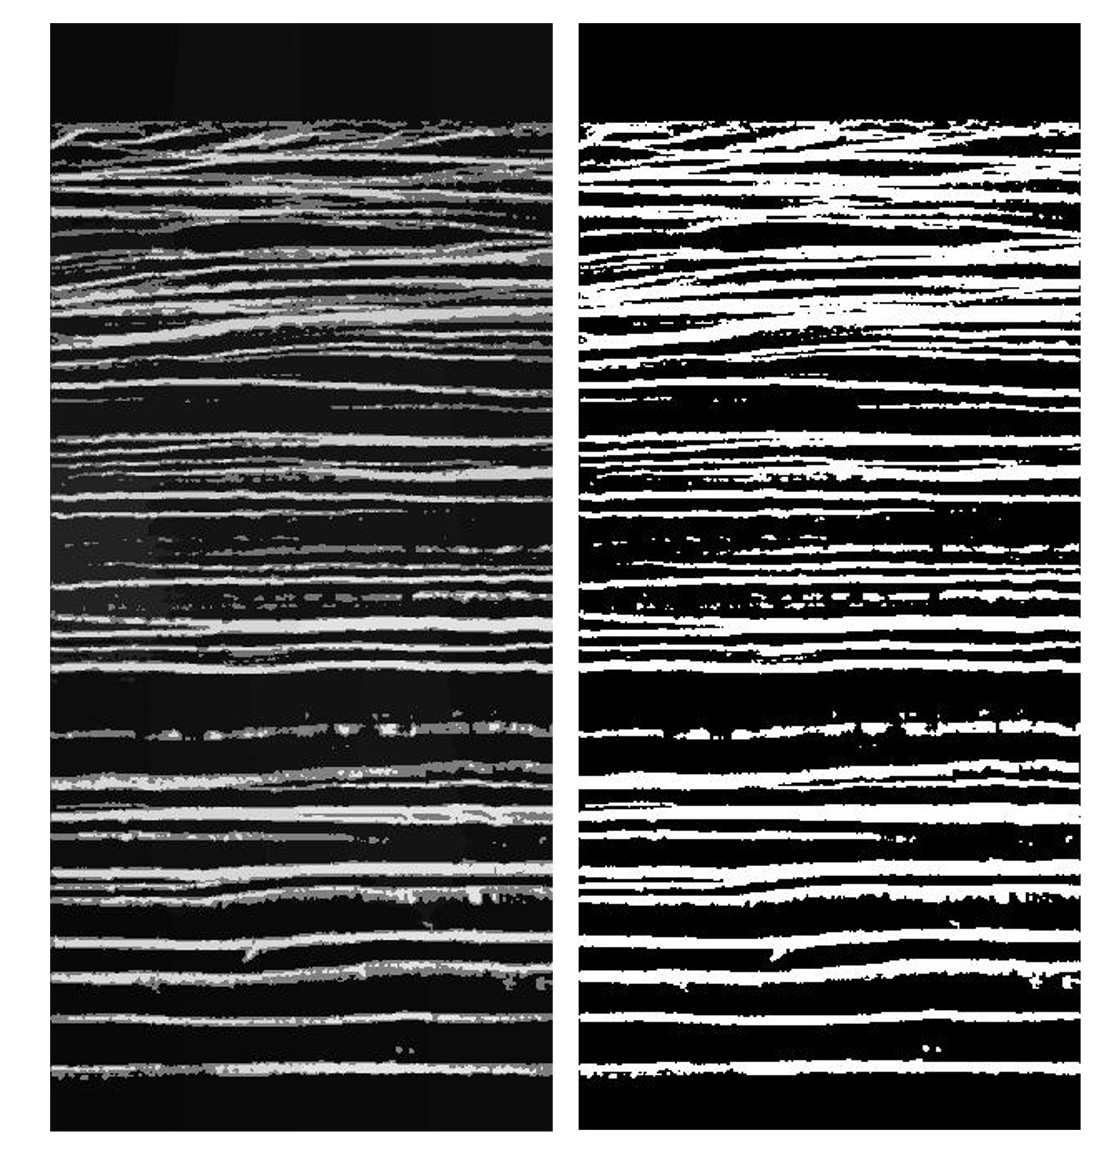
\includegraphics[height=5in]{complex_k_MeansResults.jpg}
\caption{k-Means result when k=30 and (x,y,brightness) are the points}
\end{figure}

\subsection{EM Algorithm}
I tried the EM algorithm. I used the same initial procedure as the more complex k-Means where I made points that consisted of a normalized x and y as well as brightness value. Instead of calling k-Means to do the clustering, I called the EM algorithm for Gaussian Mixture Models. I used external code for calling the EM algorithm. In the file emScript.m is a link to the webpage on the Matlab file exchange where I obtained the code. \\
\\
Unfortunately, the EM algorithm did not perform better than k-means. It did not bring out the thin fibers in the top very well and parts of other fibers that should have appeared did not seem to appear. Additionally, the unsegmented image was quite noisy and did not have nice looking clusters like what appeared with k-Means. It could be that the EM algorithm is meant to be used when the distribution follows a Gaussian model, whereas this data set may not really be following that model. Due to poor initial results and the fact that the data is not likely following a Gaussian mixture model, I decided not to try the route of improving the EM algorithm results. \\
\\
I used imagesc to display the raw clusters which resulted from running the EM algorithm. Here is the result which was noisier than desired:
\begin{figure}[H]
\centering
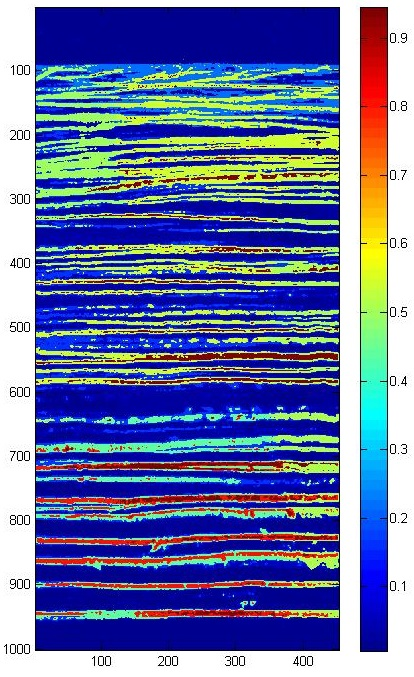
\includegraphics[height=5in]{emResultUnsegmented.jpg}
\caption{The resultant clusters from running EM}
\end{figure}
I then used a classification boundary of $0.25$ on the result and any cluster above that was given a white color while clusters below that were given a black color value. I did trial and error to see the optimal classification boundary on the EM result and $0.25$ gave me the best result, hence why it is that instead of $0.3$ like before. Here is the result where fibers were not brought out as well as hoped:
\begin{figure}[H]
\centering
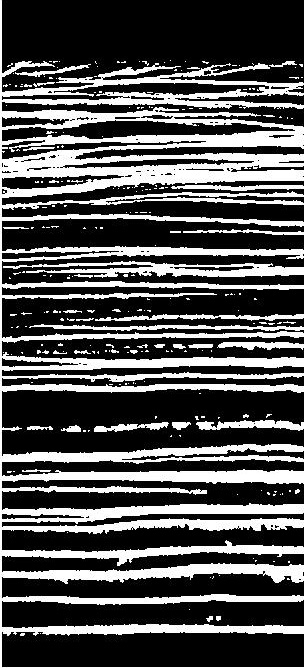
\includegraphics[height=5in]{emResultSegmented.jpg}
\caption{The resultant clusters from running EM segmented}
\end{figure}

\subsection{Min-cut algorithm on Markov Random Fields}
I tried using the MRF model to separate out the fibers. I used the min-cut code that I did for an earlier homework. It performed well at selecting certain fibers but it did not select all the fibers that I wanted it to. This could have happened because the min cut algorithm is optimized for selecting foreground and background. The fibers do not quite have the image properties of a foreground in that they are not all in one region of the image, so using min cut is not as effective. Perhaps if I had done the algorithm but with one seed point per fiber region then it might have worked well. Unfortunately, the number of fiber regions is not always known. Since there is a large number of images in each data set, having to figure out the number of regions is impractical. Thus, it would have not been worth trying to continue making the MRF model work well with my data set. Here is the result of using it which shows that some of the fibers have been located but not all of them. \\
\begin{figure}[H]
\centering
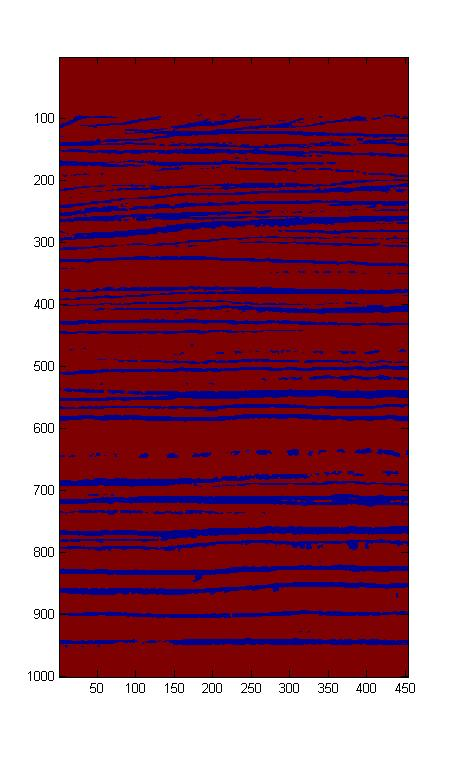
\includegraphics[height=5in]{minCutResult.jpg}
\caption{The resultant segmentation after using min-cut}
\end{figure}

\subsection{Object Correlation}
I finally tried object correlation. I tried a few different templates. I used one template that was just a little square where a fiber was located. I also tried a larger middle square that had a few fibers. Unfortunately, when I did the correlation and then displayed the results as an image, it just looked like a blurrier version of the old image in both cases. It did not bring out the fibers in the way I was hoping. \\
\\
I did also think about using correlation for alignment. I was thinking that I would correlate two images with the same template and I could see where the highest correlation was in both images and match up those points. Unfortunately, the results were not reliable enough to be useful in that the two points did not match up well enough. \\
\\
Correlation likely failed due to differences in the fibers in size, shape, and thickness, making them hard to detect with a single template. I did not try to use a HOG approach but it is not likely to produce great results due to the variations mentioned above. In addition to the variation in fibers themselves, many of the fiber objects will diverge into two separate fibers or there will be fibers that will converge into one fiber. These variations in shape are important to detect but make it even harder to use correlation. \\
\\
In the end, due to the variations mentioned above, object detection using correlation does not seem like a practical route to pursue to improve the clustering. When I looked at the other data sets, I noticed that the fibers there are even more different than the ones in the rabbit set, so the same issues would appear again.\\
\\
Below is an illustration of the correlation results when using the small template. The results are seen for the first two images and it can be observed that the fibers are not brought out too well. Additionally, the points with the highest correlation do not correspond too well to be used for alignment.
\begin{figure}[H]
\centering
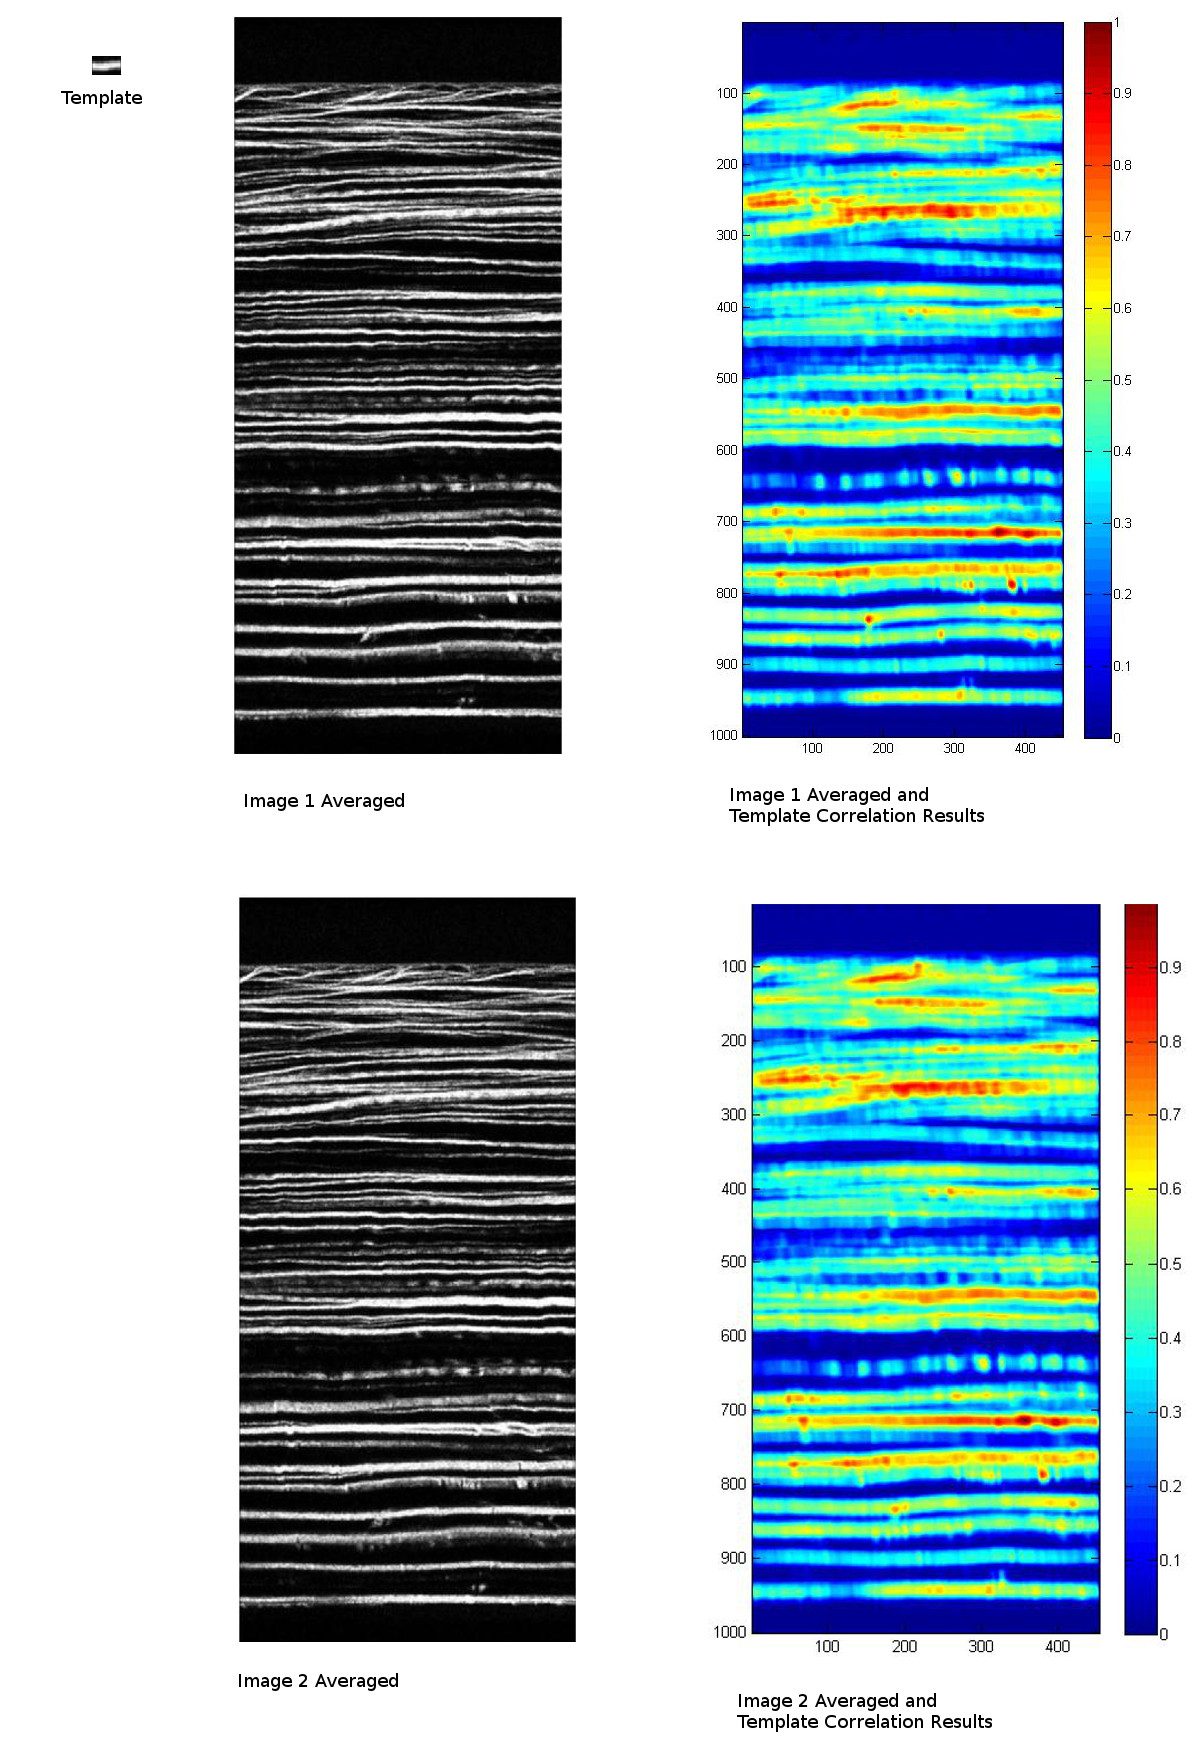
\includegraphics[height=9in]{correlationResults_template1.jpg}
\caption{The correlation results on image1 and image2 using template 1}
\end{figure}
I was hoping that the results would be better with a bigger template, but as can be observed below, they were not.
\begin{figure}[H]
\centering
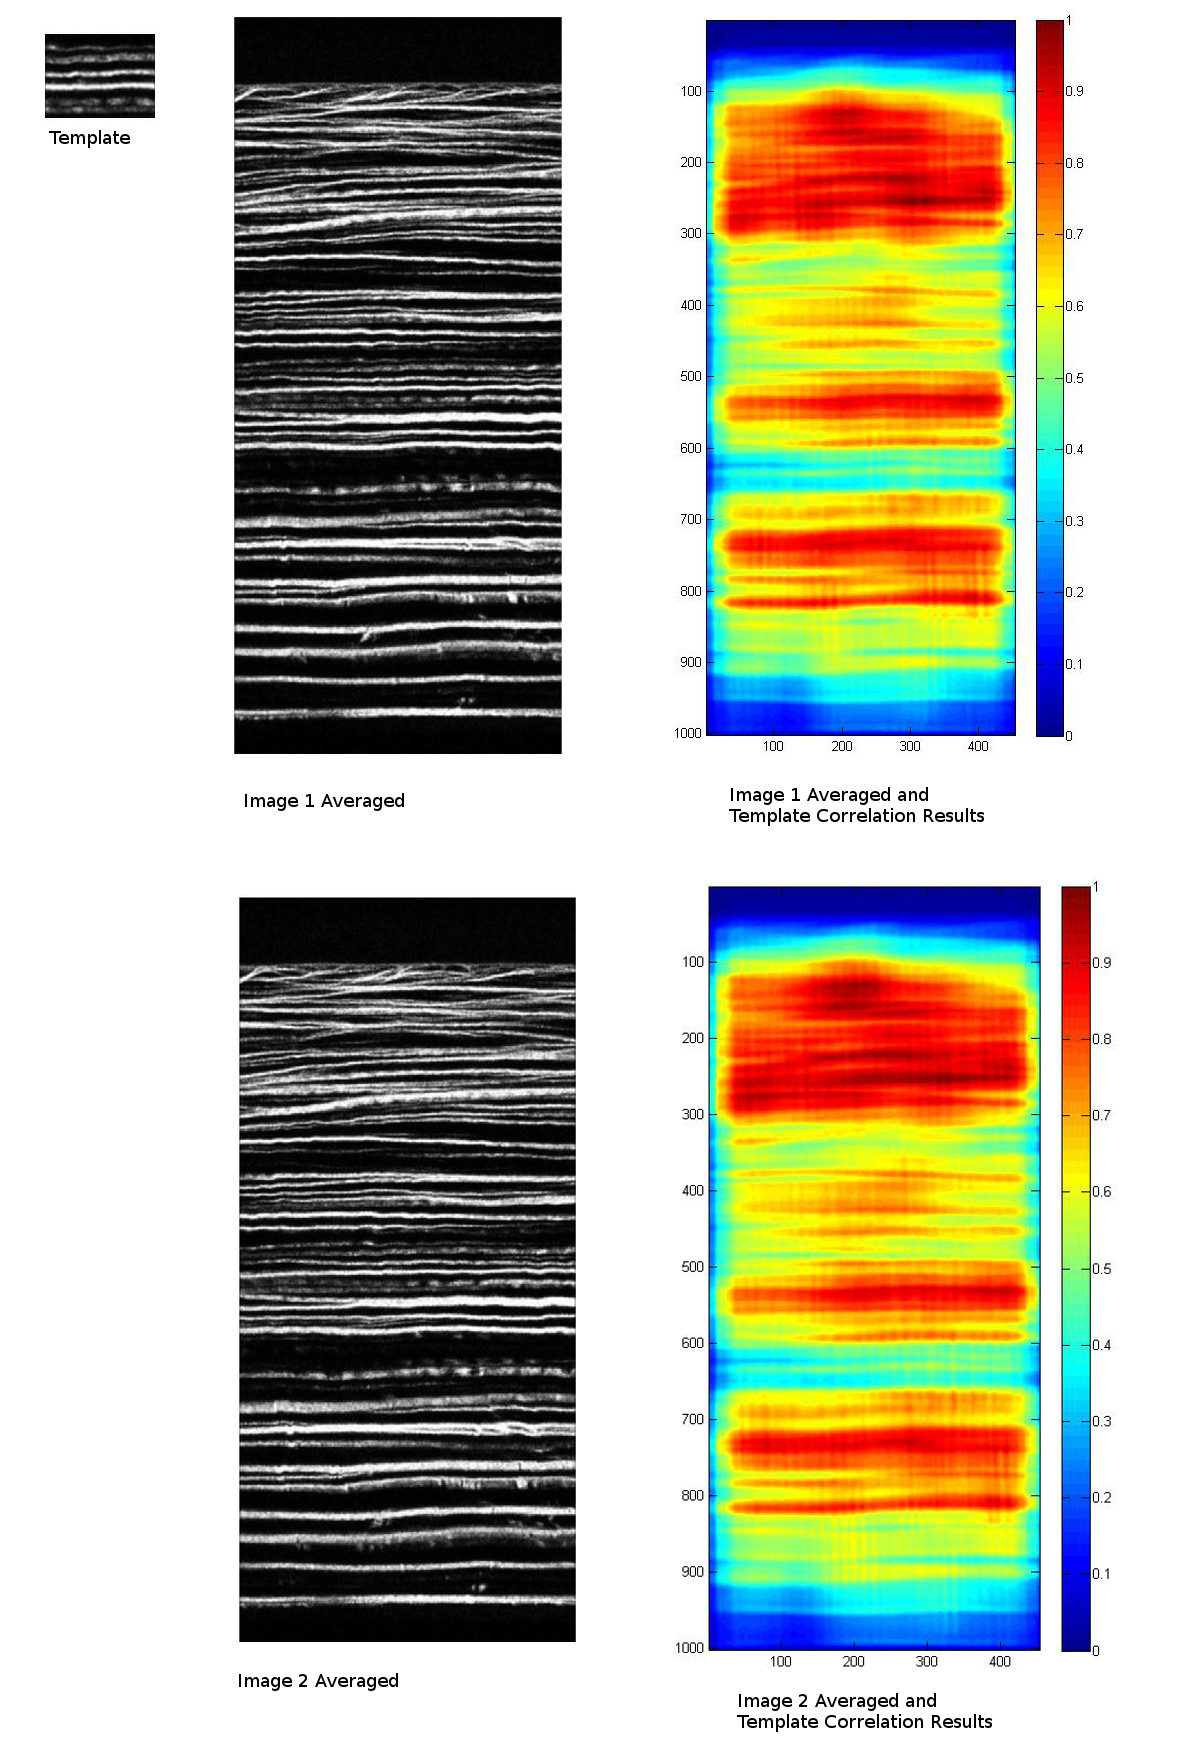
\includegraphics[height=9in]{correlationResults_template2.jpg}
\caption{The correlation results on image1 and image2 using template 1}
\end{figure}

\section{Smoothing of Segmented Images}

Lastly, after applying k-Means to segment the images, I wanted to smooth out the segmented images to make the fibers look better. I tried a few different filters and in the end, a median filter followed by a bilateral filter proved to be the best option. I liked the result of using a median filter as it takes out noisy pixels and does not use them in any computation. I used a bilateral filter because it is both noise reducing and edge preserving and takes into account both spatial proximity and brightness when doing the averaging. In this way, it was really good at bringing out the fibers. When I implemented bilateral filtering, I used Matlab code from the Matlab file exchange. 
\begin{figure}[H]
\centering
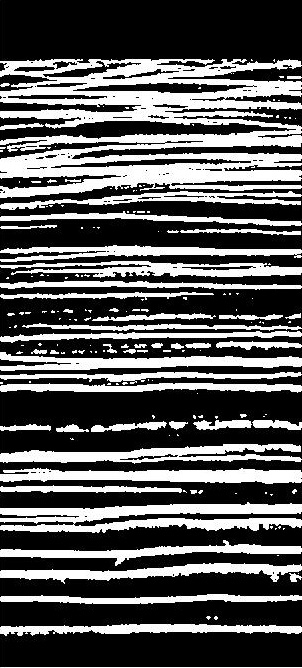
\includegraphics[height=5in]{image1_medianFilterResult.jpg}
\caption{Result of applying median filter to segmented image}
\end{figure}

\begin{figure}[H]
\centering
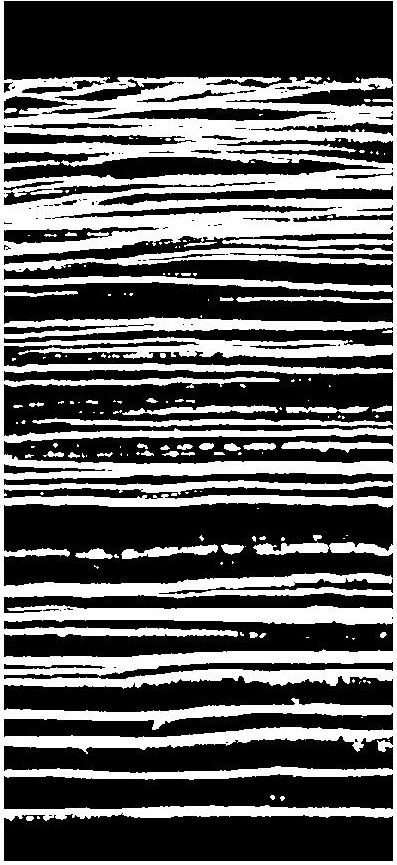
\includegraphics[height=5in]{image1_bilateralFilterResult.jpg}
\caption{Result of applying bilateral filter to the median filtered image}
\end{figure}

\section{Making the Data Set}

This section describes what was done once the images were segmented. 

\subsection{Alignment}

I had images taken at different depths but I was not told that that they should be overlaid on top of each other so I tried to see if it would make sense if the images should be shifted slightly as I make the 3D data set. \\
\\
I took an image and shifted it on top of another image. I then took the overlap region for both images and considered a pixel a fiber if both of them had fibers there. Each of the overlap regions were different sizes so I made sure to normalize the number of matches by the total number of pixels. Even after doing this, the most overlap occurred when you did not do any shifting. \\
\\
As mentioned above, I thought about using correlation and matching up the top points between two images but my results were not reliable enough for that. I thought about whether I could use another method to find points and then match them up but due to the variations in the fibers, there does not seem to be a reliable way of doing that. Thus in the end I decided not to use any special alignment and just put the images together. 

\subsection{Displaying the Data Set}

After determining that doing a normal overlay was the best route, I decided to bring out the fibers even more by adding images between each pair that consisted of pixels where both images had fibers. I then took all the images generated and put them together in a 3D data set. I used the volume renderer VolView (http://www.kitware.com/opensource/volview.html) to view the 3D data set that I generated from the segmented images. Here is a screenshot of it displaying the volume rendering:
\begin{figure}[H]
\centering
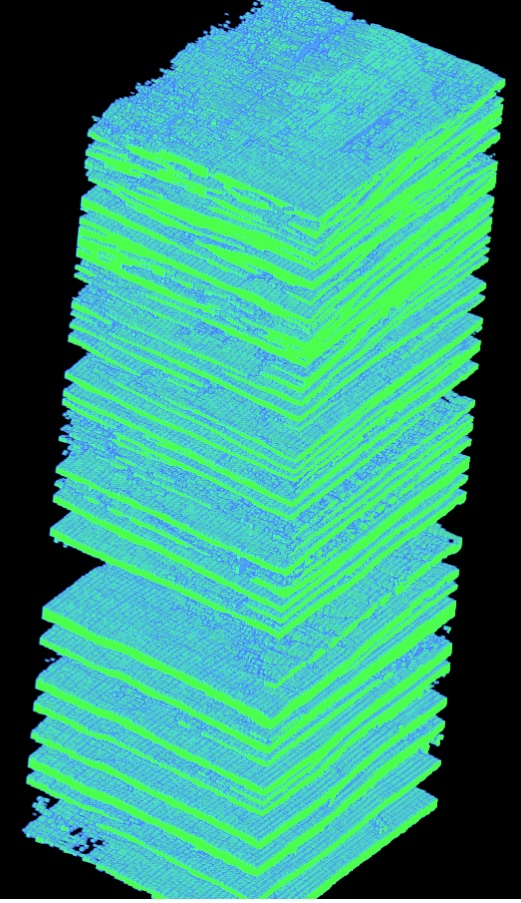
\includegraphics[height=5in]{volumeRendering.jpg}
\caption{Volume Rendering screenshot}
\end{figure}

\section{Results and Future Work}

After all was said and done, I ended up with a nice looking rendering of the collagen fibers in a rabbit cornea. I showed it to the Ophthalmologists and they thought it was a good first step in using 3D visualization to analyze the fibers. There were thin fibers at the top and I was especially pleased that those were brought out very well. Using techniques from this course allowed me to bring out the fibers very well. The volumetric rendering would have been hazy and uninformative had I not done any segmentation on the images. Since the fibers were brought out, I will be able to do isosurface extraction to make them into a mesh. \\
\\
The pictures above show a data set of collagen fibers for the cornea of a rabbit. There are other data sets that we were given. I ran the above algorithms on them but the segmentation was not as successful. The above tools turned out to be the ideal choice and their parameters were tuned for the rabbit data set. Since the other data sets have images that look different though, a different set of tools and parameters with those tools are required. In addition to finding a different set of tools for segmenting a different data set, there is work to be done on improving the current segmentation. There are also further things we plan to do with the 3D data. 

\subsection{Work on improving segmentation}

Qualitatively, my results seemed good and the ophthalmologists seemed to think they looked nice, but there is definitely room to improve the segmentation. When evaluating a clustering, I ended up relying on my subjective comparison between the clustered image and the original image to decide how well the fibers were brought out. It would be great if I could get a few preliminarily segmented images to compare my results with so that I can have a quantitative evaluation of how well the clustering performed. I could then compare the error rates that the various methods produce and use whichever method has the least error overall. \\
\\
It has come to our attention that when there are spots that are lined up in the image, there is likely a fiber there. We will use this and make sure to use a clustering method that favors cases where that happens. 
\\

\subsection{Work on 3D reconstruction}

The Ophthalmology department really liked seeing the fibers in the data set and their concern lies with analyzing these fibers. They want to know how many fibers there are and how they branch off each other as well as know their shape and size. In order to enable this type of analysis, the next step then will be to take the 3D data set and generate a series of meshes for the isosurface that corresponds to a voxel value of 1. This will give us a mesh for each of the fibers that we can then move around, analyze, and run simulations on.  


\end{document}








